
\subsection*{6.2 Combination of Events}
In probability, events can be combined using the **addition law** (for "or" situations) and the **multiplication law** (for "and" situations). Events can also be classified as **mutually exclusive** or **independent**.

\textbf{Key Concepts:}
\begin{itemize}
	\item \textbf{Addition Law of Probability:} Used for the probability of either event A or event B occurring.
	\[
	P(A \cup B) = P(A) + P(B) - P(A \cap B).
	\]
	\begin{center}
		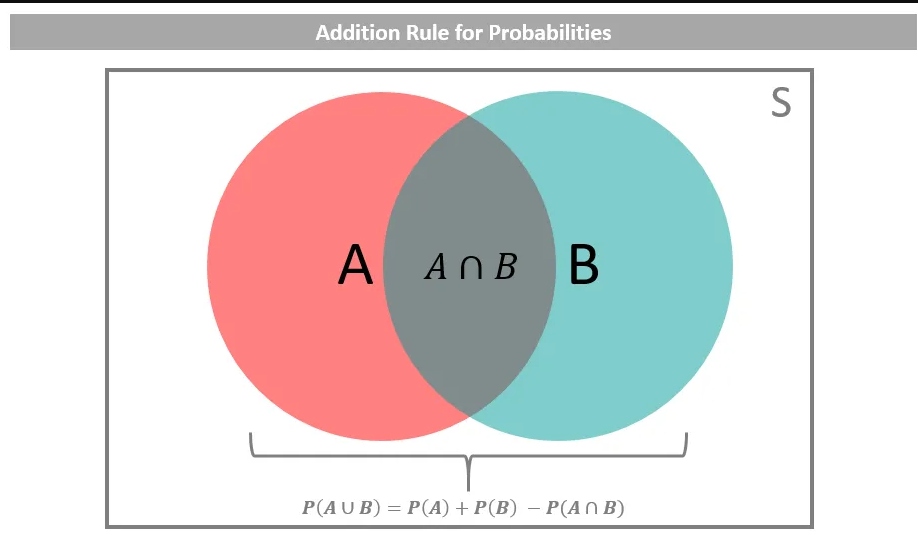
\includegraphics[width=0.6\textwidth]{6.1.png}
	\end{center}
	
	
	
	\item \textbf{Mutually Exclusive Events:} Two events that cannot happen at the same time.
	\[
	P(A \cap B) = 0.
	\]
	If A and B are mutually exclusive, then:
	\[
	P(A \cup B) = P(A) + P(B).
	\]
	
	\item \textbf{Independent Events:} The occurrence of one event does not affect the probability of the other.
	\[
	P(A \cap B) = P(A) \times P(B).
	\]
\end{itemize}

\textbf{Examples:}

\begin{flushleft}
	\textbf{Example 1: Addition Rule with Overlapping Events}
	
	A deck of 52 cards contains 13 hearts and 13 face cards. If a card is drawn at random, what is the probability that it is a heart or a face card?
	
	\textbf{Solution:}
	
	Step 1: Use the addition formula:
	\[
	P(A \cup B) = P(A) + P(B) - P(A \cap B).
	\]
	
	Step 2: Find the probabilities:
	\[
	P(\text{Heart}) = \frac{13}{52}, \quad P(\text{Face Card}) = \frac{12}{52}.
	\]
	
	Since there are 3 face cards in hearts, 
	\[
	P(\text{Heart} \cap \text{Face Card}) = \frac{3}{52}.
	\]
	
	Step 3: Compute:
	\[
	P(\text{Heart or Face Card}) = \frac{13}{52} + \frac{12}{52} - \frac{3}{52} = \frac{22}{52} = \frac{11}{26}.
	\]
\end{flushleft}

\begin{flushleft}
	\textbf{Example 2: Probability of Independent Events}
	
	A fair die is rolled, and a coin is flipped. What is the probability of getting a 4 on the die and heads on the coin?
	
	\textbf{Solution:}
	
	Step 1: Identify the probabilities:
	\[
	P(\text{Rolling a 4}) = \frac{1}{6}, \quad P(\text{Flipping Heads}) = \frac{1}{2}.
	\]
	
	Step 2: Since these are independent events, use the multiplication rule:
	\[
	P(4 \cap H) = P(4) \times P(H) = \frac{1}{6} \times \frac{1}{2} = \frac{1}{12}.
	\]
\end{flushleft}

\begin{flushleft}
	\textbf{Example 3: Mutually Exclusive Events}
	
	A bag contains 5 red marbles and 7 blue marbles. If one marble is drawn at random, what is the probability that it is either red or blue?
	
	\textbf{Solution:}
	
	Since drawing a red marble and drawing a blue marble are mutually exclusive events, we use:
	\[
	P(A \cup B) = P(A) + P(B).
	\]
	
	\[
	P(\text{Red}) = \frac{5}{12}, \quad P(\text{Blue}) = \frac{7}{12}.
	\]
	
	\[
	P(\text{Red or Blue}) = \frac{5}{12} + \frac{7}{12} = 1.
	\]
	
	Since one of these must occur, the probability is 1.
\end{flushleft}

\begin{flushleft}
	\textbf{Example 4: Probability of Winning Independent Contracts}
	
	A building contractor tendered for two independent contracts, $X$ and $Y$. The probabilities that he will win contract $X$ is 0.5 and not win contract $Y$ is 0.3. What is the probability that he will:
	
	\begin{enumerate}
		\item Win both contracts?
		\item Win exactly one of the contracts?
		\item Win neither of the contracts?
	\end{enumerate}
	
	\textbf{Solution:}
	
	Let:
	\[
	P(X) = 0.5, \quad P(\text{Not } Y) = 0.3.
	\]
	Since $P(\text{Not } Y) = 0.3$, then:
	\[
	P(Y) = 1 - 0.3 = 0.7.
	\]
	
	\textbf{(i) Probability of Winning Both Contracts:}
	
	Since the events are independent:
	\[
	P(X \cap Y) = P(X) \times P(Y) = 0.5 \times 0.7 = 0.35.
	\]
	
	\textbf{(ii) Probability of Winning Exactly One Contract:}
	
	This occurs in two ways:
	- Wins $X$ and loses $Y$: $P(X \cap \text{Not } Y) = P(X) \times P(\text{Not } Y)$.
	- Loses $X$ and wins $Y$: $P(\text{Not } X \cap Y) = P(\text{Not } X) \times P(Y)$.
	
	Since $P(\text{Not } X) = 1 - 0.5 = 0.5$, we compute:
	\[
	P(X \cap \text{Not } Y) = 0.5 \times 0.3 = 0.15.
	\]
	
	\[
	P(\text{Not } X \cap Y) = 0.5 \times 0.7 = 0.35.
	\]
	
	Adding both cases:
	\[
	P(\text{Exactly one contract}) = 0.15 + 0.35 = 0.50.
	\]
	
	\textbf{(iii) Probability of Winning Neither Contract:}
	
	\[
	P(\text{Not } X \cap \text{Not } Y) = P(\text{Not } X) \times P(\text{Not } Y).
	\]
	
	\[
	= 0.5 \times 0.3 = 0.15.
	\]
	
	\textbf{Final Answers:}
	\begin{itemize}
		\item Probability of winning both contracts: $0.35$.
		\item Probability of winning exactly one contract: $0.50$.
		\item Probability of winning neither contract: $0.15$.
	\end{itemize}
\end{flushleft}

